% g(z,y)=y^2-z: two sheets, with one regular local graph in the dashed box.
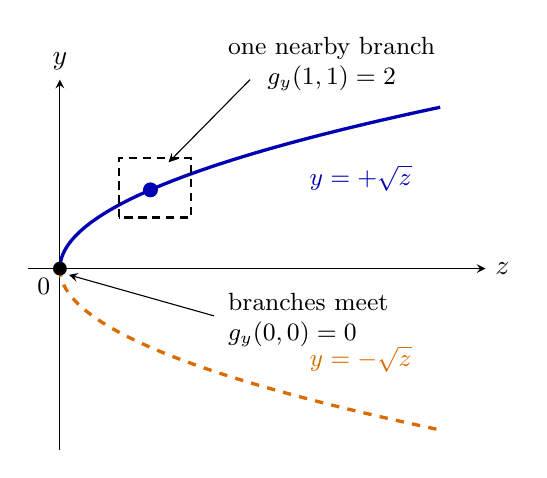
\begin{tikzpicture}[>=stealth,x=1.15cm,y=1cm]
\draw[->,black](-.35,0)--(4.7,0)node[right]{$z$};
\draw[->,black](0,-2.3)--(0,2.4)node[above]{$y$};
\draw[blue!70!black,very thick,domain=0:2.05,samples=80,variable=\t]plot({\t*\t},\t);
\draw[orange!85!black,very thick,dashed,domain=0:2.05,samples=80,variable=\t]plot({\t*\t},-\t);
\node[blue!70!black,anchor=west,font=\small]at(2.65,1.15){$y=+\sqrt z$};
\node[orange!85!black,anchor=west,font=\small]at(2.65,-1.15){$y=-\sqrt z$};
\draw[densely dashed,thick](.65,.65)rectangle(1.45,1.4);
\fill[blue!70!black](1,1)circle(2.7pt);
\draw[->] (2.1,2.4)--(1.2,1.35);
\node[font=\small,align=center]at(3,2.6){one nearby branch\\$g_y(1,1)=2$};
\fill[black](0,0)circle(2.5pt);
\draw[->] (1.7,-.6)--(.1,-.08);
\node[font=\small,align=left,anchor=west]at(1.75,-.65){branches meet\\$g_y(0,0)=0$};
\node[below left,font=\small]at(0,0){$0$};
\end{tikzpicture}
